% MODELO CONEM 2016
\documentclass[10pt,fleqn,a4paper]{article}
\usepackage{abcm}
\begin{document}
    
    % CABEÇALHO
    \fancypagestyle{firststyle}
	{
   		\lhead{\emph{Anais do XXIII Encontro de Iniciação Científica e Pós-Graduação do ITA -  XXIII ENCITA / 2017 Instituto Tecnológico de Aeronáutica, São José dos Campos, SP, Brasil, XXIII  26 de outubro de 2017}}  
	}
    \thispagestyle{firststyle}
    \vspace{-.5cm}
    \hspace{-.8cm}
    \begin{tabular}{p{\textwidth}}
    \begin{center}
    \vspace{-.6cm}
    \title{Controle de motor elétrico Brushless Maxon 45fl-200142 para robô jogador de futebol Small Size}
    \end{center}
    \textbf{Aloysio Galvão Lopes}\\
    \small{Instituto Tecnológico de Aeronáutica}\\
    \small{Rua H8C, 322, DCTA}\\
    \small{12.228-462 - São José dos Campos/SP}\\
    \small{Bolsista PIBIC - CNPq}\\
    \small{aloysiogl@gmail.com}\\
    \\ 
    \textbf{Carlos César Aparecido Eguti}\\
    \small{Instituto Tecnológico de Aeronáutica}\\
    \small{Centro de Competência em Manufatura}\\
    \small{Praça Marechal Eduardo Gomes, 50}\\
    \small{12.229-900 – São José dos Campos / SP}\\
    \small{cesar.eguti@gmail.com}\\
    \\ 
    \textbf{Marcos Ricardo Omena de Albuquerque Maximo}\\
    \small{Instituto Tecnológico de Aeronáutica}\\
    \small{Divisão de Ciência da Computação}\\
    \small{Praça Marechal Eduardo Gomes, 50}\\
    \small{12.229-900 – São José dos Campos / SP}\\
    \small{maximo.marcos@gmail.com}\\
%    \authors{Nome do primeiro autor, e-mail$^1$} \\
%    \authors{Nome do segundo autor, e-mail$^1$} \\
%    \authors{Nome do terceiro autor, e-mail$^2$} \\\\
%    \institution{$^1$Nome da instituição, endereço para correspondência} \\
%    \institution{$^2$Nome da instituição, endereço para correspondência} \\
%    \\
%    \authors{\textcolor[rgb]{0.98,0.00,0.00}{Mesmo  formato para outros autores e instituições, se houver.}} \\
    \\
    \abstract{\textbf{Resumo:}
     Neste trabalho é realizada a simulação e implementação de um controle do motor elétrico do tipo Brushless Maxon 45fl-200142. O objetivo do trabalho foi realizar o modelamento matemático das equações que regem o motor citado; realizar a simulação do modelo obtido; desenvolver, simular e otimizar os parâmetros de um controlador PI; desenvolver o hardware para o controle do motor e implementar o controlador para o motor.
     
     Para isso, foi, inicialmente, projetado e criado o hardware para controle do motor. Em seguida, o hardware foi testado em um motor BLDC de drive de DVD em loop aberto. Após isso, foi realizada a modelagem do motor baseada nos parâmetros físicos fornecidos pelo fabricante; com base nisso, foi possível simular o comportamento do motor e projetar o controlador. Por fim, foi possível implementar o controlador no hardware desenvolvido e controlar o motor Maxon 45fl-200142.
     
     Dos resultados obtidos, foi possível concluir que o controle do motor só pode ser realizado com feedback. Isso significa que o controle do motor do drive de DVD em loop aberto não obteve sucesso. No entanto, o controle do motor Maxon foi realizado com sucesso, pois foi utilizado feedback dos sensores de efeito Hall, além do mais os resultados de velocidade angular obtidos pelo motor se mantiveram fiéis ao modelo, o que mostra que o modelo utilizado descreve adequadamente o motor.}\\    
     \keywords{\textbf{Palavras-chave:} Motor elétrico Brushless, Modelagem física, Simulação, Controle de velocidade.}\\
    \end{tabular}
    

    \section{INTRODUÇÃO}
    A ITAndroids, equipe de robótica do ITA, é uma iniciativa de alunos do ITA que representa a instituição em diversas competições de robótica nacionais e internacionais. O principal objetivo dessa iniciativa é a integração dos alunos com atividades de pesquisa em engenharia, em especial em robótica e inteligência artificial.
    
    A ITAndroids acredita que o hardware é fundamental no desenvolvimento de qualquer projeto de robótica, por isso, recentemente tem-se investido bastante no desenvolvimento dessa área. O desenvolvimento de conhecimento na área de controle de motores elétricos, assim, torna-se fundamental para a melhoria técnica da iniciativa.
    
    Nesse sentido, abre-se caminho para a participação na categoria Small Size, a qual necessita de uma eletrônica mais desenvolvida o que implica diretamente no desenvolvimento de conhecimento sobre controle de motores. Os motores utilizados para a locomoção dos robôs são motores Brushless, essa escolha se justifica pelo fato de que motores Brushless (sem comutadores mecânicos do tipo escova) são mais eficientes, ocupam menos espaço e apresentam desgaste muito menor que motores DC tradicionais.
    
    Uma vez que o desgaste mecânico durante as partidas de futebol de robôs Small Size é elevado e é preciso alto rendimento dos sistemas mecânicos: os motores Brushless, também chamados BLDC são a escolha ideal; além disso, as principais equipes internacionais fazem uso de desses motores. Como principal exemplo temos a equipe tailandesa SKUBA, descrita em \cite{skuba}, na qual se baseia o projeto mecânico do Small Size da ITAndroids. Em contrapartida, o controle deste tipo de atuador mecânico se dá de maneira mais complexa, uma vez que a comutação do campo magnético não é feita mecanicamente por escovas. A Figura \ref{fig:esquemamotor}, abaixo, ilustra a mecânica de um motor BLDC.

	\begin{figure}[ht]
		\begin{center}
			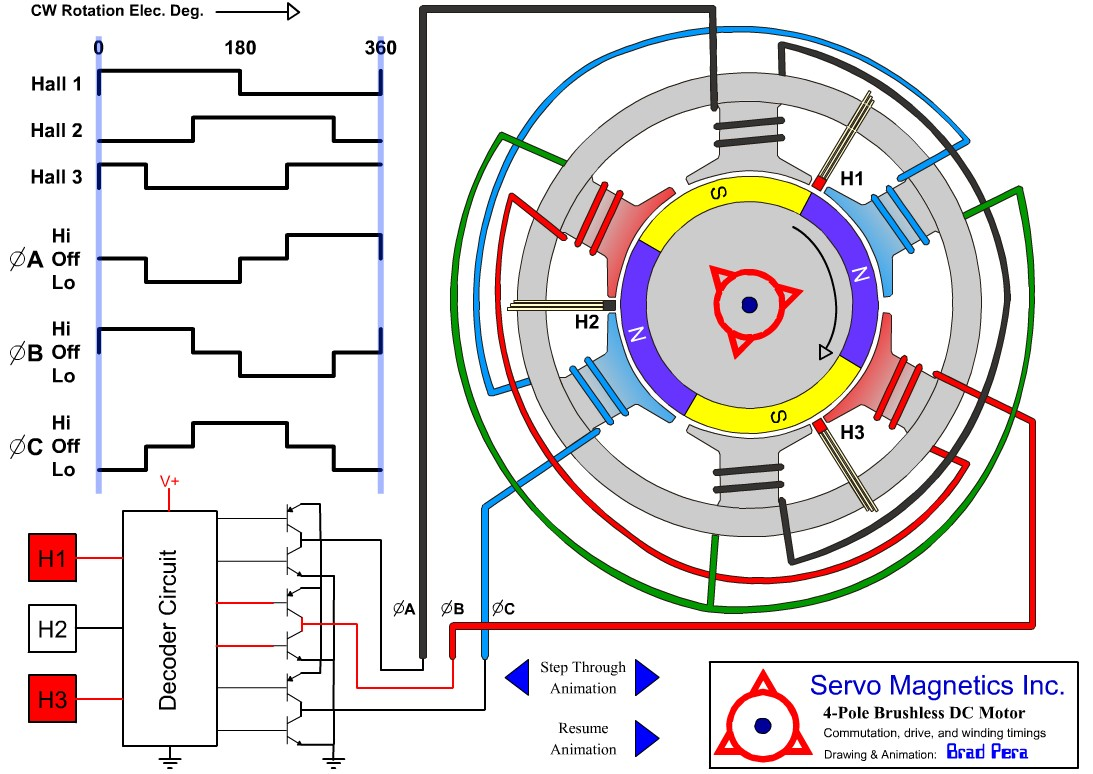
\includegraphics[angle=0, scale=0.2]{images/4-Pole-brushless-DC-motor-animation}
		\end{center}
		\caption{\textbf{Esquema completo de um motor elétrico Brushless trifásico.}}
		\label{fig:esquemamotor}
	\end{figure}
    
    O controle da comutação do campo magnético para esse tipo de motor é feito eletronicamente, seguindo o procedimento descrito em \cite{introducaobldc}, o que acarreta que seja necessário que um dispositivo eletrônico, tal como um microcontrolador, fique dedicado ao controle de cada um dos quatro motores do robô Small Size. Isso aumenta a complexidade do sistema de locomoção como um todo, no entanto traz diversos ganhos em eficiência para o projeto.
    
    Nesse sentido, busca-se, aqui, modelar o motor Maxon 45fl-200142 e ser capaz de realizar a comutação eletronicamente. Adicionalmente, deseja-se, simular e implementar um controlador PI.
    
    \section{MODELAGEM DO MOTOR}
    \subsection{Funcionamento do Motor Elétrico Brushless Maxon 45fl-200142}
    
    Um motor elétrico Brushless têm várias possíveis configurações, no entanto, a configuração trifásica ganha destaque em eficiência. Isso pode ser constatado pela grande preferência no mercado por tal tipo de motor BLDC. O motor aqui estudado é de configuração trifásica, logo, há três entradas cada uma para uma bobina do motor.
    
    Isso significa que existem três fases diferentes que devem ser eletronicamente comutadas para que se obtenha a rotação do motor. Além disso, o ciclo de rotação do motor é composto de seis etapas distintas, portanto o motor rotaciona com uma comutação de seis passos. Há apenas uma sequência correta de seis combinações das fases do motor para cada sentido de rotação. Pode-se, no entanto, encontrar sequências de comutação distintas das duas principais que rotacionam o motor. Comutações com essas sequências resultam em menor eficiência e perda de precisão na rotação, por isso, é essencial encontrar as sequências corretas de comutação.
    
    Vale destacar, como já dito, que cada fase corresponde a uma bobina do motor e que estas bobinas estão interligadas. Assim, cada passo corresponde a aplicar tensão entre dois terminais de duas bobinas. As bobinas podem estar distribuídas ao redor da carcaça do motor como pode ser notado na Fig. \ref{fig:esquemamotor}, o que faz que uma rotação mecânica completa não seja equivalente a um ciclo elétrico (ciclização entre os seis passos de comutação). No caso do motor estudado, são necessárias 48 comutações para que uma revolução completa seja atingida; isso, portanto, significa que a cada oito ciclos elétricos ocorre um ciclo mecânico no motor. A figura \ref{fig:comutacao}, abaixo, ilustra a comutação de fases em um motor BLDC.

	\begin{figure}[ht]
		\begin{center}
			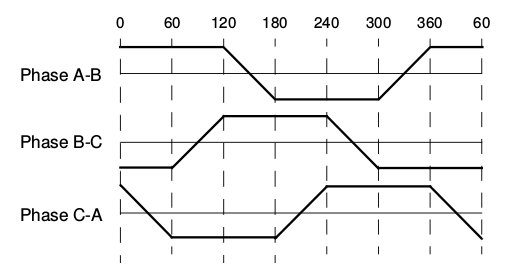
\includegraphics[angle=0, scale=0.5]{images/comutacao}
		\end{center}
		\caption{\textbf{Contra eletromotriz nas três fases de um motor BLDC comutando. Retirado de \cite{introducaobldc}.}}
		\label{fig:comutacao}
	\end{figure}
    
    
    Adicionalmente, é comum haver três sensores de efeito Hall (como é o caso deste motor), para que seja possível controlar a comutação com feedback. A combinação das três saídas de cada um dos sensores de efeito Hall dá a próxima comutação do motor de maneira única para cada sentido de rotação. Com isso, pode-se montar uma tabela de correspondências entre saídas do sensores de efeito Hall e passo de comutação: a tabela de comutação do motor. Essa tabela, em geral, não é fornecida pelo fabricante e deve ser montada para que seja possível controlar o motor.
    
    \subsection{Modelamento do Motor}
    
    O modelo matemático utilizado no estudo do motor BLDC é o mesmo modelo utilizado para um motor DC convencional, o qual, em termos práticos, é uma boa aproximação. Um modelamento completo pode ser encontrado em \cite{modelomotor}. Considera-se que o torque produzido pelo motor é proporcional à corrente como mostrado em Eq. (\ref{torquemotor}) e que a tensão no motor é proporcional à velocidade angular $\dot{\theta}$, como mostrado em Eq. (\ref{tensaomotor}).
    
    \begin{equation}
    \tau = K_ti \label{torquemotor}
    \end{equation}
    \begin{equation}
    V = K_b\dot{\theta} \label{tensaomotor}
    \end{equation}
    
    Considerando, ainda, o momento de inércia do motor $J$ e que existe um atrito viscoso $b\dot{\theta}$, pela terceira lei de Newton, chega-se à Eq. (\ref{leidenewtonmotor}). Utilizando a lei das malhas e considerando a queda de tensão devido à resistência do motor, à sua indutância e à conversão da energia em energia mecânica, sendo $\varepsilon$ a tensão da fonte, chega-se à Eq. (\ref{malhasmotor}).
    
    \begin{equation}
    J\ddot{\theta} = K_ti - b\dot{\theta} \label{leidenewtonmotor}
    \end{equation}
    \begin{equation}
    \varepsilon = K_b\dot{\theta} + L\frac{di}{dt} + Ri \label{malhasmotor}
    \end{equation}
    
    Pode-se, associando Eq. (\ref{leidenewtonmotor}) e Eq. (\ref{malhasmotor}), chegar à função de transferência do motor, mostrada abaixo em Eq. (\ref{plantamotor}). Observa-se que foram utilizados os dados fornecidos em \cite{Datasheet} pelo fabricante e foram desconsiderados os termos do atrito viscoso, pois eram negligenciáveis.
    
    \begin{equation}
    \frac{\dot{\Theta}(s)}{\varepsilon(s)} = \frac{13.095}{2.66 \cdot 10^{-6} s^2+0.0171s+1} \label{plantamotor}
    \end{equation}
    
    \section{HARDWARE}
    
    Foi confeccionado um hardware para acionamento do motor baseado no esquema mostrado abaixo, em Fig \ref{fig:diagrama}, descrito em \cite{atmeldiagrama}. 
    
	\begin{figure}[ht]
		\begin{center}
			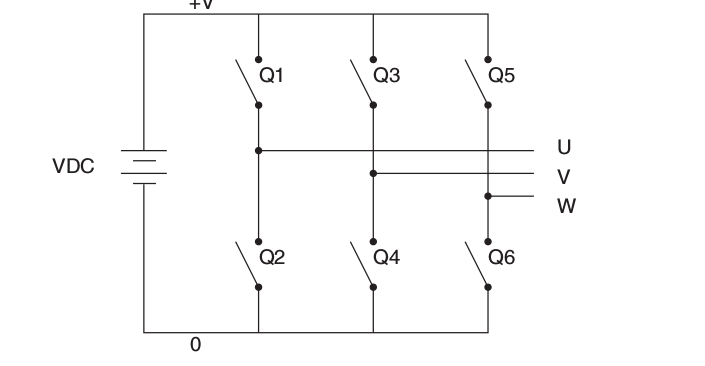
\includegraphics[angle=0, scale=0.5]{images/circuitdiagram}
		\end{center}
		\caption{\textbf{Diagrama do circuito para acionamento do motor. Retirado de \cite{atmeldiagrama}.}}
		\label{fig:diagrama}
	\end{figure}
    
    Foram utilizados seis pares darlington TIP 122 para montar o esquema mostrado acima de três meias pontes H e uma placa de desenvolvimento Arduino$^{\small{TM}}$ Mega ADK para o controle. O sistema inicialmente foi testado com um motor Brushless retirado de um drive de DVD em loop aberto. Observou-se que sem um feedback dos sensores a velocidade máxima atingida pelo motor era muito pequena e a rotação não se dava de maneira suave. Isso mostra que sem informações sobre a posição do rotor, este facilmente não é capaz de acompanhar a variação do campo magnético.
    
    Abaixo, é mostrada na Figura \ref{fig:montagemcircuito} a montagem do circuito para o controle do motor. Na Figura \ref{fig:motorantigo}, é mostrado o motor de drive de DVD utilizado inicialmente.

	\begin{figure}[ht]
		\begin{center}
			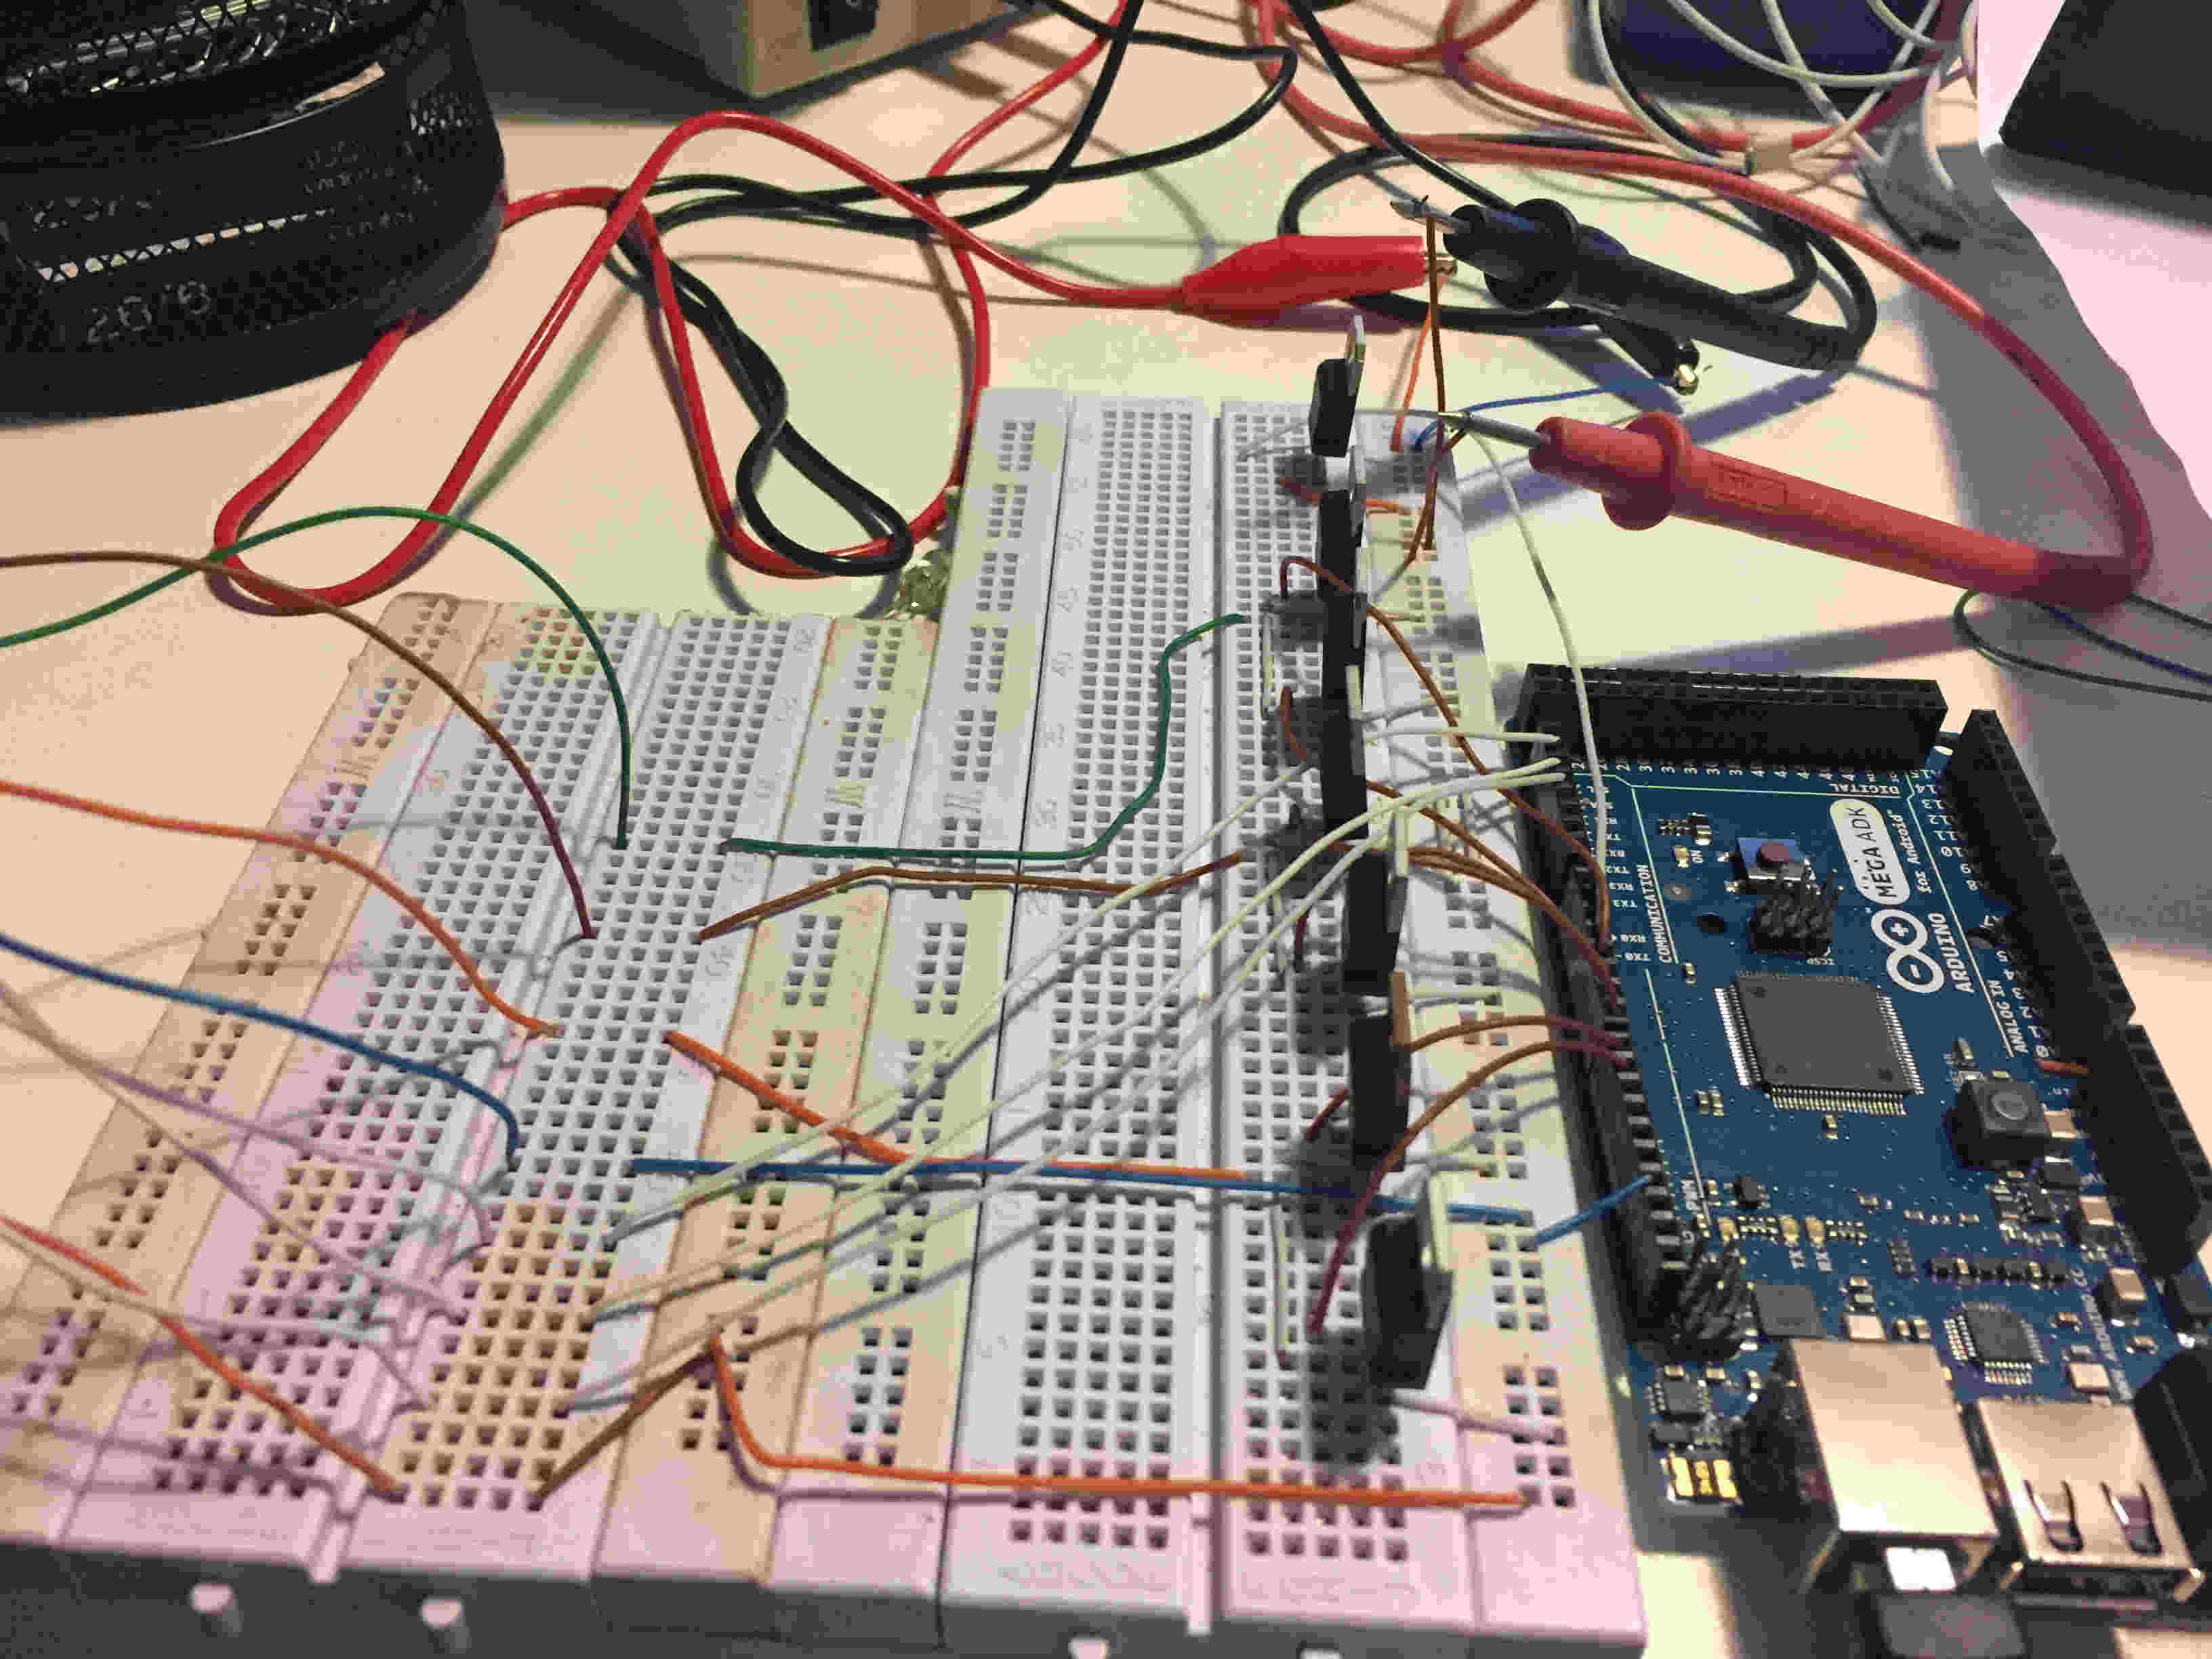
\includegraphics[angle=0, scale=0.06]{images/montagemcircuito}
		\end{center}
		\caption{\textbf{Figura da montagem do circuito para controle do motor.}}
		\label{fig:montagemcircuito}
	\end{figure}

	\begin{figure}[ht]
		\begin{center}
			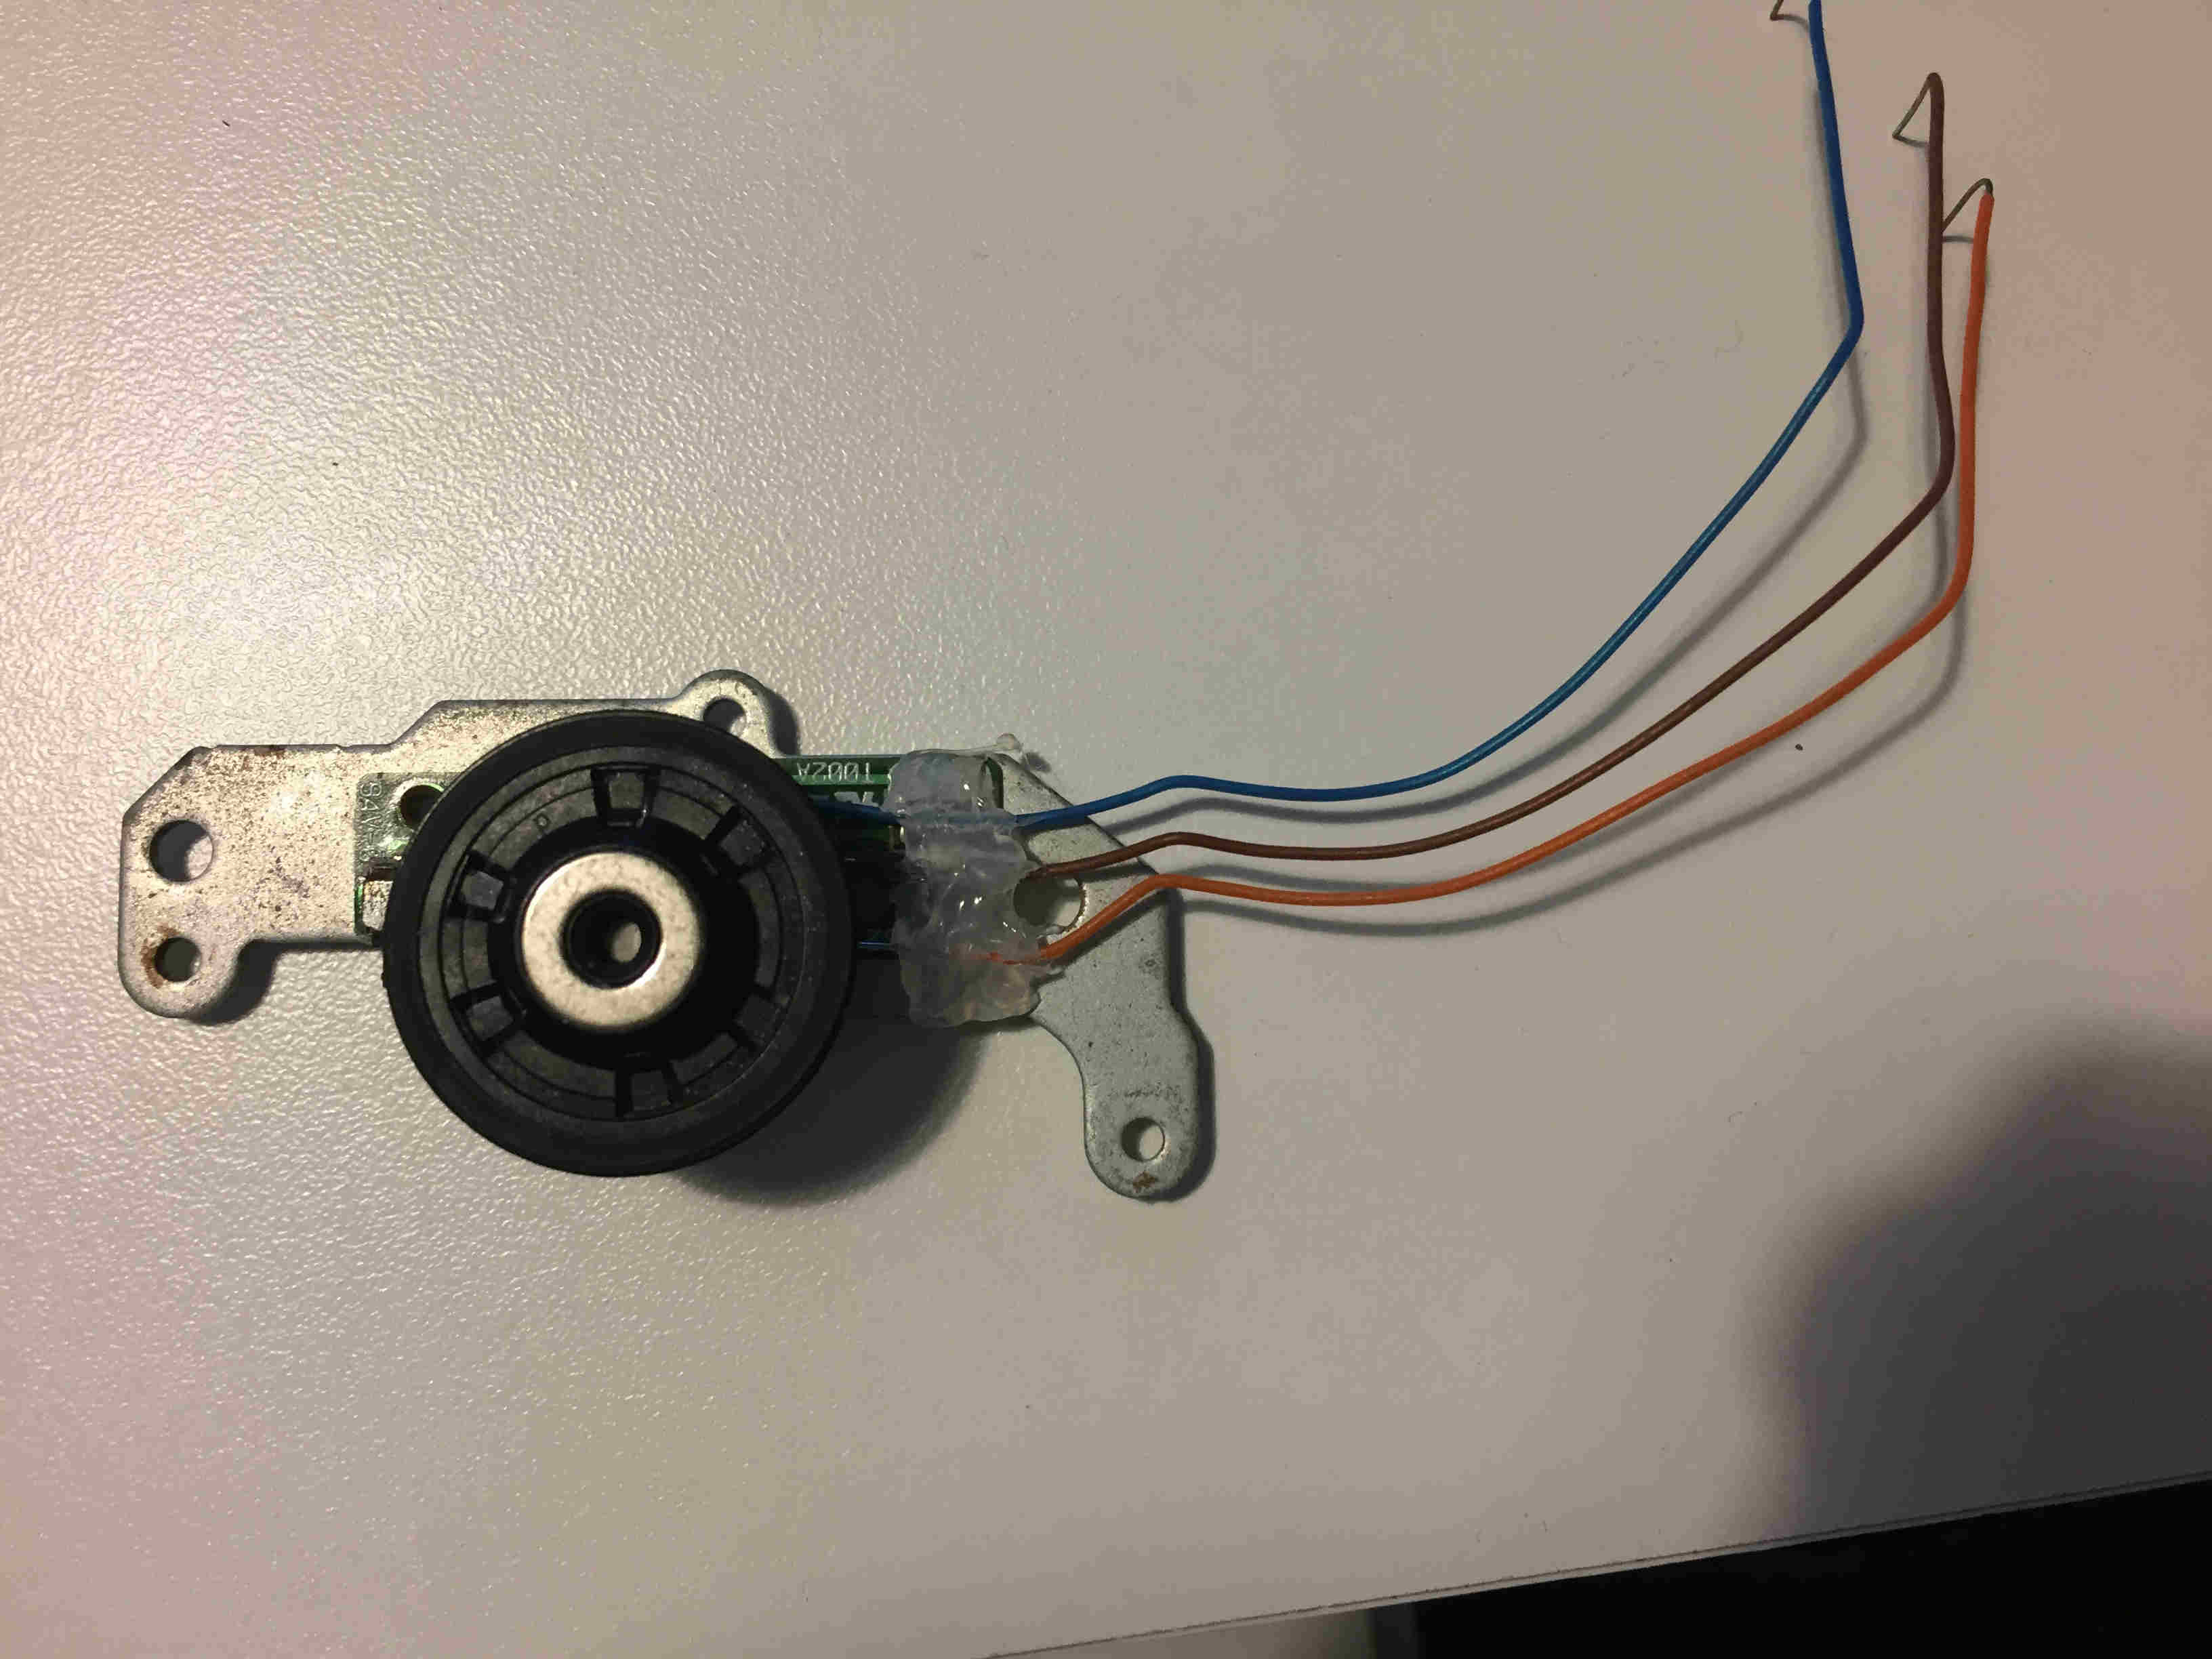
\includegraphics[angle=0, scale=0.06]{images/motorantigo}
		\end{center}
		\caption{\textbf{Motor de drive de DVD utilizado nos testes, nota-se que não há saídas para sensores de efeito Hall.}}
		\label{fig:motorantigo}
	\end{figure}
    
    Em uma segunda etapa, utilizou-se o motor Maxon 45fl-200142, cujo controle é o objetivo deste estudo. Nesse caso, foi possível utilizar o feedback dos sensores de efeito Hall e obter uma rotação suave, além disso, foi desenvolvido um script para a obtenção da tabela de comutação, uma vez que esta não é fornecida pelo fabricante. O que este script faz é ciclizar lentamente (1s) as saídas do motor conforme descrito na sequência de comutação direta em \cite{atmeldiagrama} e, em seguida, fazer a leitura dos sensores de efeito Hall. Com isso, é possível montar a tabela de comutação direta; a tabela inversa pe montada por meio da tabela direta, apenas invertendo a lógica de rotação.
    
    Este script pode ser, posteriormente, utilizado para a obtenção da tabela de comutação de qualquer motor Brushless com sensores de efeito Hall. Vale ressaltar que a regulação da velocidade aqui é feita utilizando PWM. Para isso, uma saída PWM é gerada para cada transistor que leva corrente do motor ao ground, seguindo o esquema mostrado em Fig. \ref{fig:diagrama}.
    A Figura \ref{fig:motornovo}, abaixo, mostra o motor da Maxon rotacionando. Mais adiante serão tratados os aspectos de controle implementados.

	\begin{figure}[ht]
		\begin{center}
			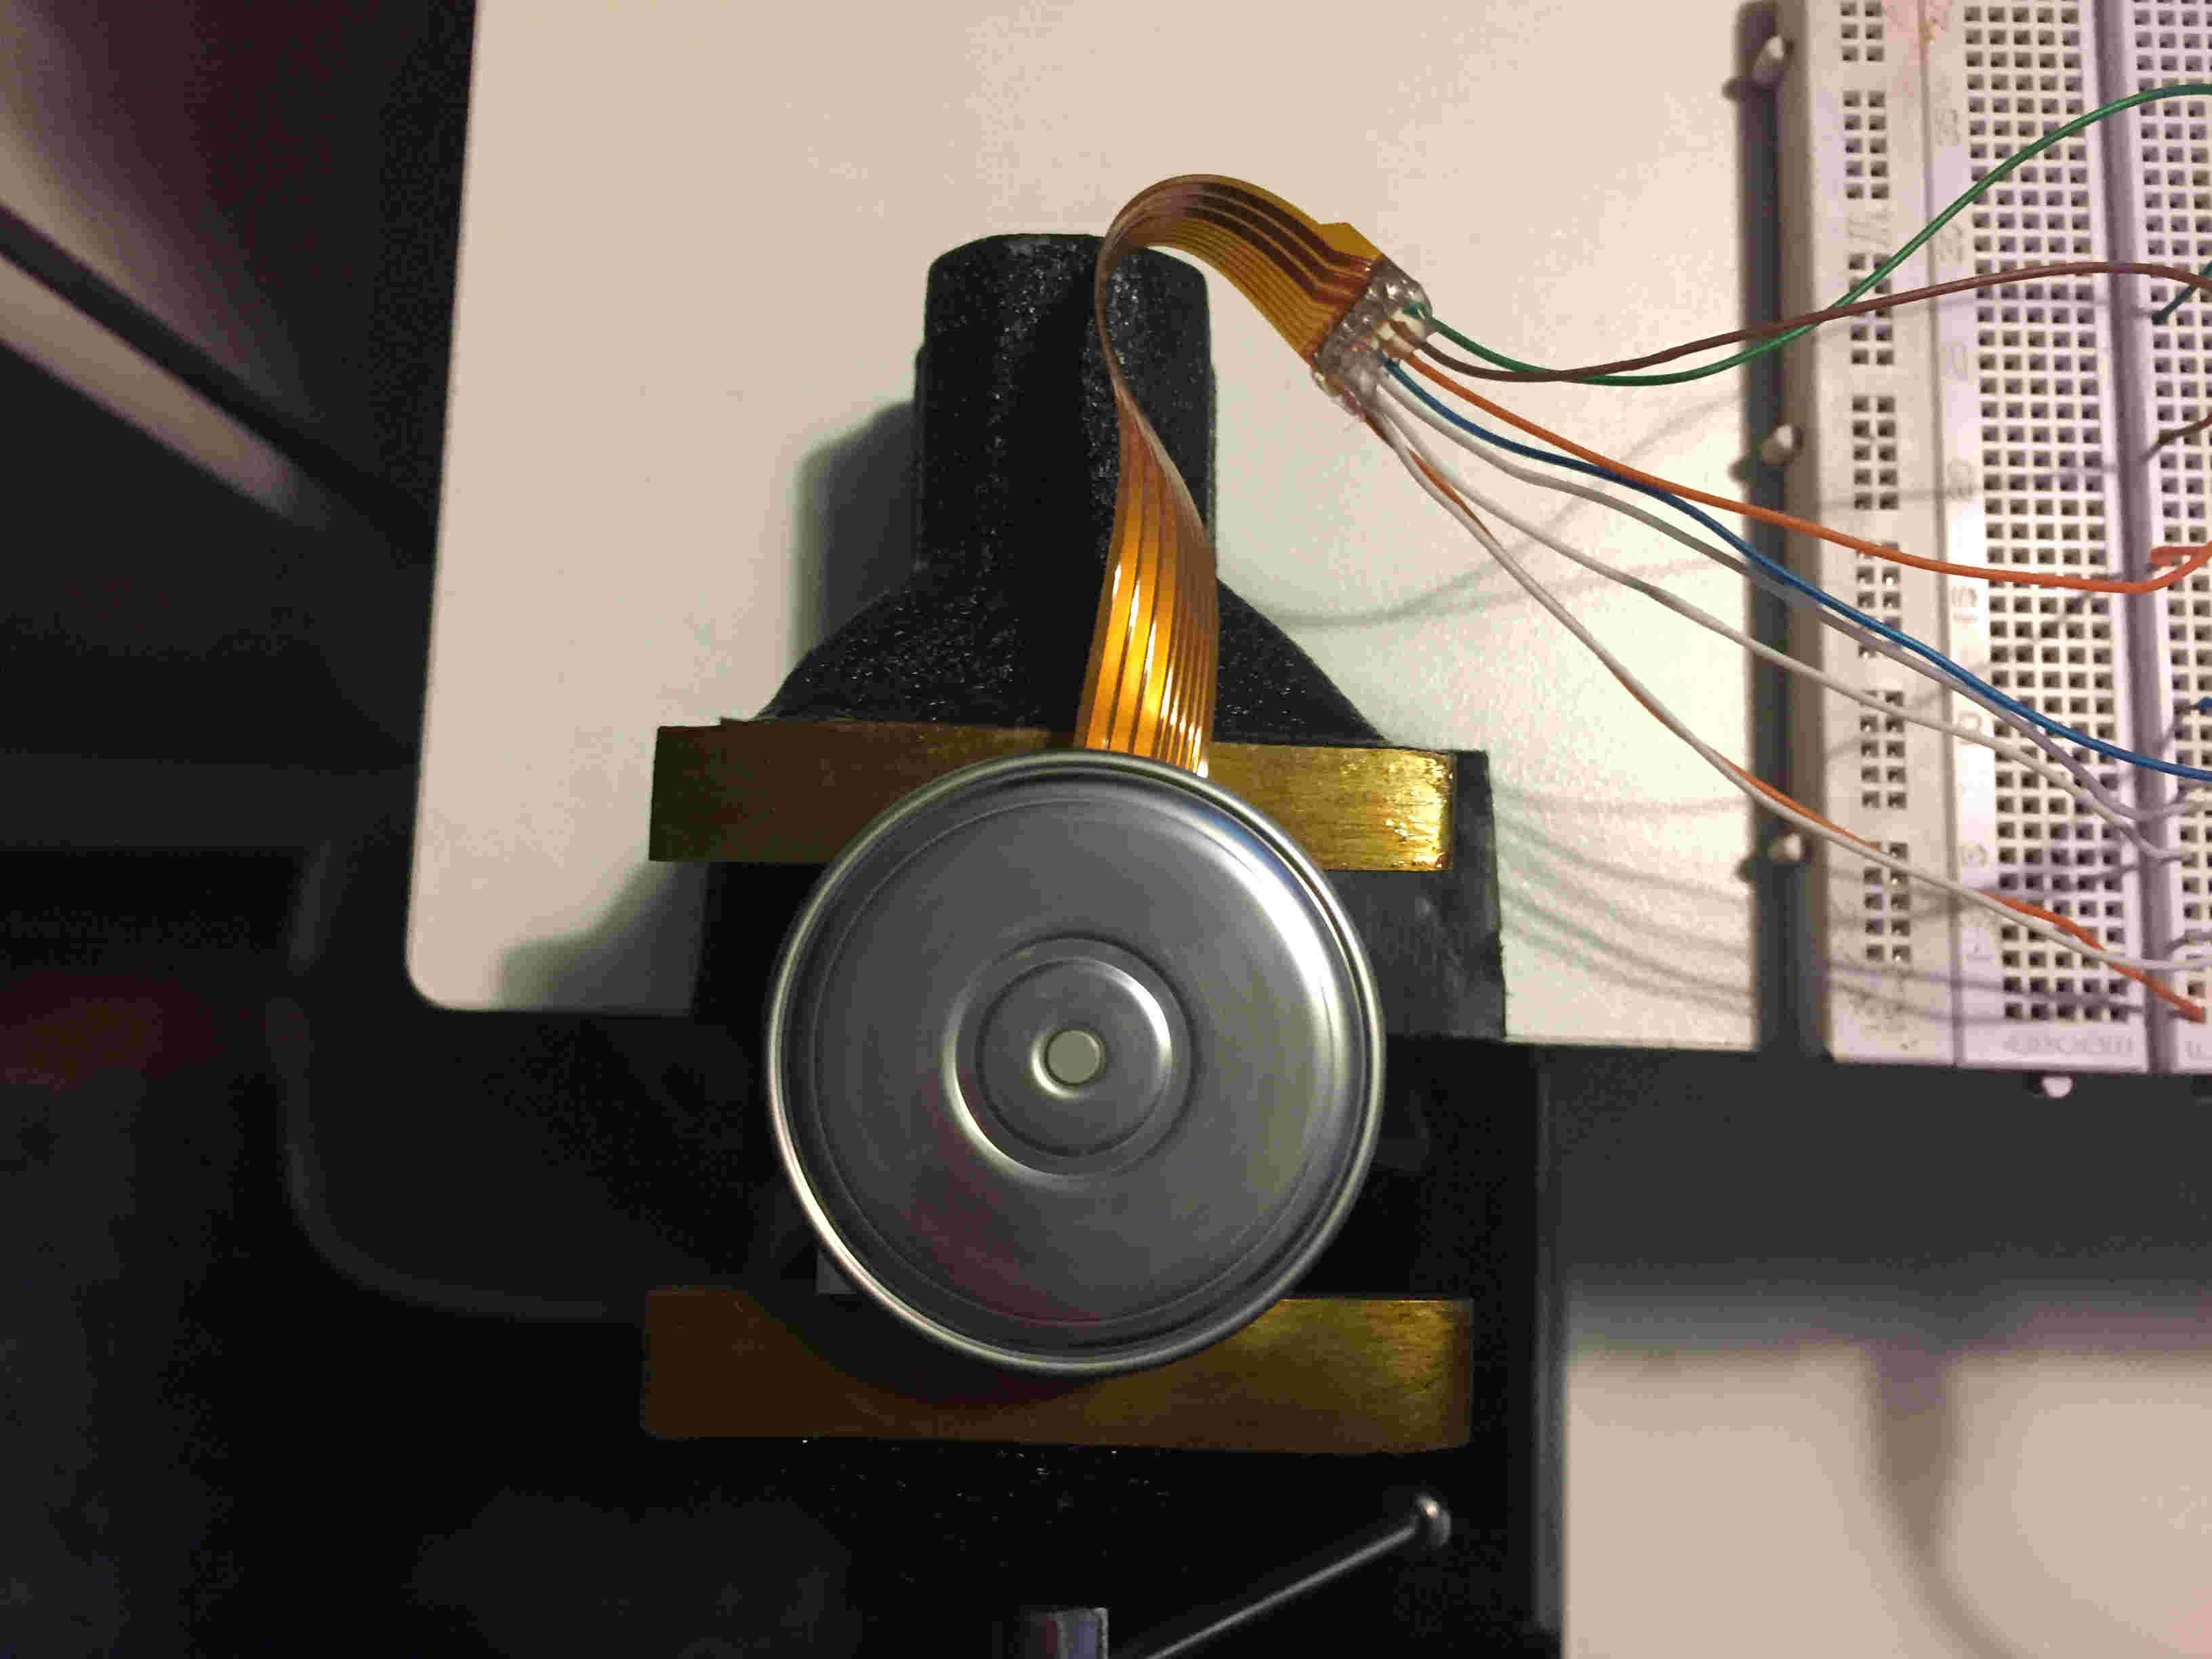
\includegraphics[angle=0, scale=0.06]{images/motornovo}
		\end{center}
		\caption{\textbf{Motor Maxon 45fl-200142 rotacionando.}}
		\label{fig:motornovo}
	\end{figure}
    
    \section{SIMULAÇÃO}
    
    Foi implementada em MATLAB$^{\small{TM}}$ a função de transferência de Eq. (\ref{plantamotor}) e, com isso, foi possível obter o gráfico para a resposta em degrau do sistema, bem como o diagrama de Bode. As figuras Fig. \ref{fig:respostaemdegrau} e Fig \ref{fig:bode}, respectivamente, representam a resposta em degrau unitário e o diagrama de Bode da planta obtidos.

	\begin{figure}[ht]
		\begin{center}
			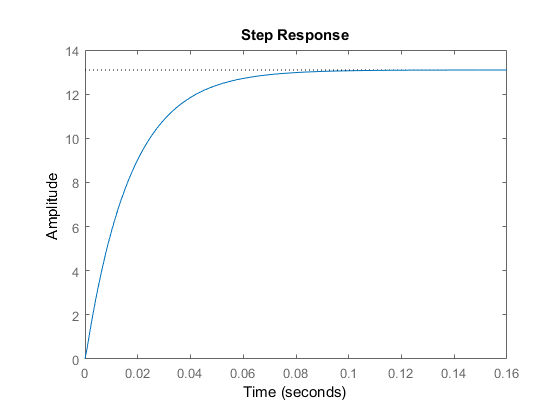
\includegraphics[angle=0, scale=0.7]{images/stepResponse}
		\end{center}
		\caption{\textbf{Análise da resposta à um degrau unitário da planta de Eq. (\ref{plantamotor}).}}
		\label{fig:respostaemdegrau}
	\end{figure}

	\begin{figure}[ht]
		\begin{center}
			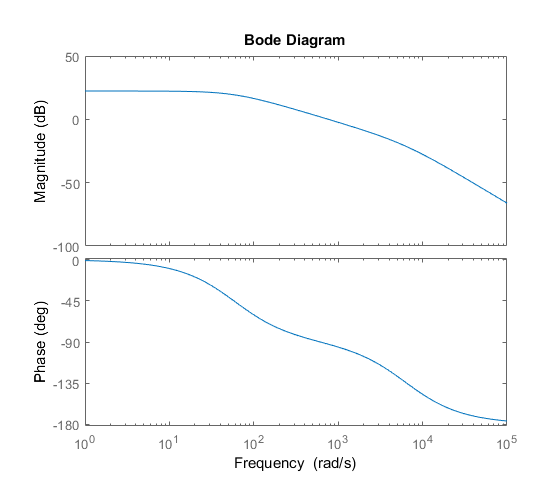
\includegraphics[angle=0, scale=0.7]{images/bode}
		\end{center}
		\caption{\textbf{Diagrama de bode para a planta de Eq. (\ref{plantamotor}).}}
		\label{fig:bode}
	\end{figure}
    
    Foi utilizado um controlador PI (proporcional e integral); esta escolha se deve ao fato de que o termo integral do controlador elimina os erros em regime. Ademais, o controle de velocidade não exige tempo de resposta elevado (como seria o caso de um controlador PD). A função de transferência em tempo contínuo para o controlador PI pode ser vista na Eq. (\ref{tfcontroladorct}).
    
    \begin{equation}
    \frac{\varepsilon(s)}{\epsilon(s)}= Kp + \frac{Ki}{s} \label{tfcontroladorct}
    \end{equation}
    
    Foi realizada uma otimização com auxílio da ferramenta de PI tunning, presente no MATLAB$^{\small{TM}}$. Buscou-se obter um pequeno overshoot e cerca de 0.001 segundo até atingir o estado estacionário. No domínio da frequência, é possível ver as fases de margem e de ganho em Fig. \ref{fig:margin}. As constantes obtidas foram: Kp = 2.8522 e Ki = 104.55. Após isso, foi gerado o gráfico de Fig. \ref{fig:saidasimulada} para a saída em velocidade angular do sistema mostrado em Fig.  \ref{fig:sistemasimulink}.
    
    \begin{figure}[ht]
    	\begin{center}
    		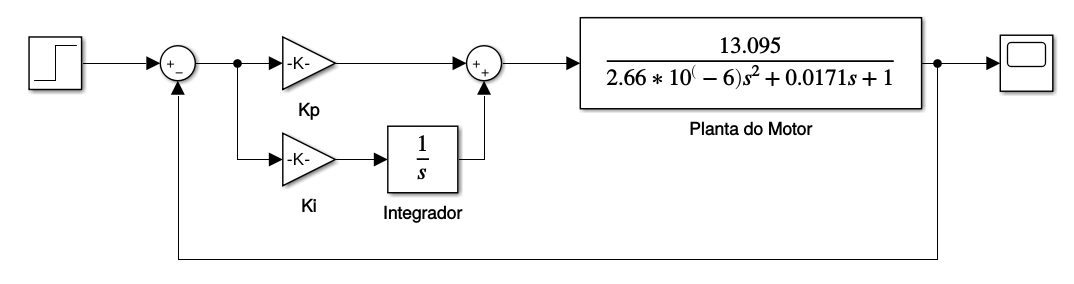
\includegraphics[angle=0, scale=0.4]{images/sistemaEControlador}
    	\end{center}
    	\caption{\textbf{Sistema completo modelado com auxílio do SIMULINK$^{\small{\textbf{TM}}}$.}}
    	\label{fig:sistemasimulink}
    \end{figure}

	\begin{figure}[ht]
		\begin{center}
			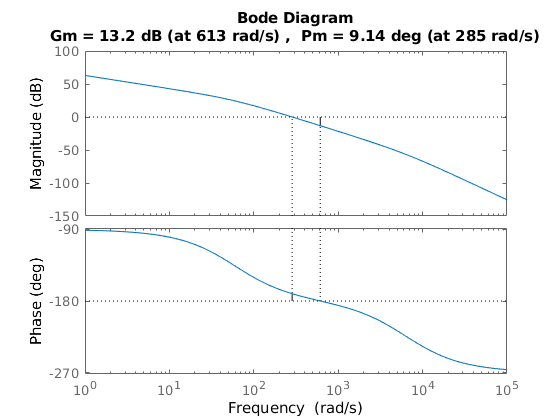
\includegraphics[angle=0, scale=0.8]{images/margins.png}
		\end{center}
		\caption{\textbf{Margens de estabilidade do sistema em estudo.}}
		\label{fig:margin}
	\end{figure}

	\begin{figure}[ht]
		\begin{center}
			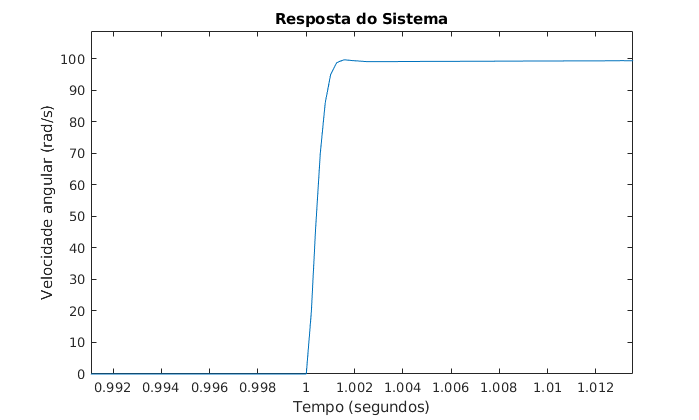
\includegraphics[angle=0, scale=0.6]{images/sistemStep}
		\end{center}
		\caption{\textbf{Saída de velocidade angular com valor fixado em 100rad/s.}}
		\label{fig:saidasimulada}
	\end{figure}
    
    Após a discretização, utilizando o método de Tustin, foi possível chegar à função de transferência discreta, mostrada em Eq. (\ref{tfdiscreta}), a qual possibilitou a implementação do controle seguindo a relação de recorrência mostrada em Eq. (\ref{recorrencia}).
    
    \begin{equation}
    \frac{\varepsilon(z)}{\epsilon(z)}= Kp + \frac{Ki T}{2}\frac{z+1}{z-1} \label{tfdiscreta}
    \end{equation}
    
    \begin{equation}
    \varepsilon[z] = \varepsilon[z-1] + Kp\cdot\epsilon[z] - Kp\cdot\epsilon[z-1] - \frac{Ki T}{2}(\epsilon[z] + \epsilon[z-1]) \label{recorrencia}
    \end{equation}
    
    \newpage
    
    \section{CONSIDERAÇÕES FINAIS}
    
    Após a implementação do algorítimo, observou-se que o motor era capaz de atingir a velocidade de 99.2 radianos por segundo, o que mostra que o modelo se adéqua aos parâmetros físicos do sistema.
    
    Ressalta-se, por fim, que existem alguns melhoramentos a serem realizados no controlador antes da implementação final no robô. Pode-se incluir uma malha de corrente, uma vez que o hardware do robô permite. Além disso, deve-se contar a inércia do robô no modelo final a ser utilizado. Os testes realizados no sistemas, também, devem ser refeitos no hardware final.
    
    Além disso, os quatro motores foram posicionados na carcaça do primeiro protótipo do robô Small Size como mostrado em Fig. (\ref{fig:smallfoto}).

	\begin{figure}[ht]
		\begin{center}
			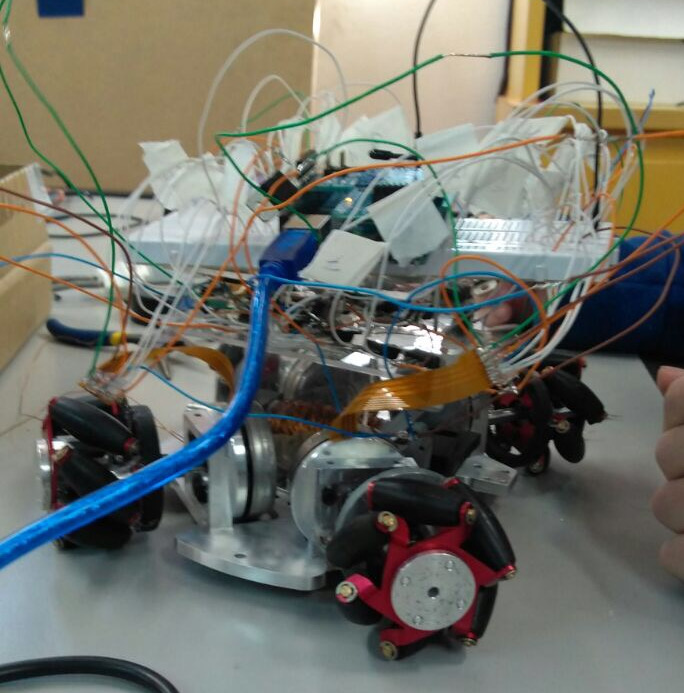
\includegraphics[angle=0, scale=0.3]{images/smallfoto}
		\end{center}
		\caption{\textbf{Fotografia do primeiro protótipo do robô Small Size com os quatro motores posicionados e operacionais.}}
		\label{fig:smallfoto}
	\end{figure}

	\section{AGRADECIMENTOS}
	
	Agradeço ao CNPQ, pelo apoio financeiro durante a realização do projeto, bem como ao meu professor orientador pelo apoio à realização do projeto. Agradeço à iniciativa ITAndroids, por fornecer os treinamentos necessários e recursos materiais para a realização do projeto.
	
	\section{REFERÊNCIAS}
	\bibliographystyle{abcm}
	\bibliography{bibliografia}
	
	\section{RESPONSABILIDADES AUTORAIS}
	
	% % RESUMO EM INGLES
	%
	\noindent{
	   \\ 
	    \begin{tabular}{||p{\textwidth}}
	    \begin{center}
	    \vspace{-.6cm}
	    \title{Maxon 45fl-200142 Brushless motor control for Small Size league soccer robot}
	    \end{center}
	    \authors{Aloysio Galvão Lopes, aloysiogl@gmail.com} \\
	    \authors{Carlos César Aparecido Eguti, cesar.eguti@gmail.com} \\
	    \authors{Marcos Ricardo Omena de Albuquerque Maximo, maximo.marcos@gmail.com} \\\\
	    \institution{Instituto Tecnológico de Aeronáutica, Rua H8C, 322, DCTA
	    	12.228-462 - São José dos Campos/SP} \\
	    \institution{Instituto Tecnológico de Aeronáutica, Centro de Competência em Manufatura
	    	Praça Marechal Eduardo Gomes, 50
	    	12.229-900 – São José dos Campos / SP} \\
	    \\
	  
	    \abstract{\textbf{Abstract:} In this work, the control of a Maxon 45fl-200142 Brushless type DC motor is simulated and implemented. The objective of the work is to develop a mathematical modeling of the equations witch rule the motor's physical behavior; perform a simulation of the model; develop, simulate and optimize the parameters of a PI controller; develop the hardware for the motor control and implement the controller for the motor.
	    	
	    To achieve this objective, initially, the hardware was projected and produced. After that the hardware was tested in a generic DVD drive Brushless motor in open loop. The next step was the modeling of Maxon's 45fl-200142 BLDC motor based in manufacturer parameters. This way it was possible to simulate the behavior of the motor and develop the controller.
	    
	    Finally, it was possible to implement the controller in the physical system and control Maxon's motor.
    	The results showed that the control of a BLDC motor can only be achieved using feedback. This means that the control of the DVD drive motor in open loop was unsuccessful. Maxon's motor control, on the other hand, was successfully achieved, because there was feedback of the Hall effect sensors, furthermore the results of angular velocity obtained were consistent with the model. This demonstrates that the utilized model describes correctly the motor.}\\
	    \keywords{\textbf{Keywords:} Electrical Brushless Motor, Physical Modeling, Simulation, Speed Control.}\\
	    \end{tabular}
	}
    
\end{document}